\section{Introduction}

Welcome to the Introduction to Computer Networks course! This course is
designed to give you a broad overview of the field of computer networks. We
will cover the basics of networking, including the physical layer, the data
link layer, the network layer, and the transport layer. We will also cover the
application layer, including the web, email, and file transfer protocols. We
will also cover some of the more advanced topics in networking, including
network security, network management, and network programming.

\subsection{Software}

\begin{center}
    
\includegraphics[width=0.3\textwidth]{images/packet_tracer.png}
\end{center}

We will use Cisco Packet Tracer to simulate the network. You can download the
software from the \href{http://www.netacad.com}{Cisco Netacad} website. The
account for each team is provided by CyberPatriot for free; you will share the
same account with your teammate.

\begin{longtable}{ccc}
    \toprule
    Team                                                     & Username                 & Password           \\
    \midrule
    $\lambda$ Lambda\footnote{Extremely good team name, no?} & cpxv.net153926@gmail.com & 6BSQ-UFPT-GE33cp15 \\
    $\psi$ Psi                                               & cpxv.net153927@gmail.com & GG6Y-XLFQ-9TSMcp15 \\
    $\mu$ Mu                                                 & cpxv.net153928@gmail.com & 5PGA-3KDT-ZMRUcp15 \\
    $\phi$ Phi                                               & cpxv.net154561@gmail.com & CTCJ-KQZH-YM2Ecp15 \\
    \bottomrule
\end{longtable}

\subsection{Hello World}

\subsubsection{Topology}

Open the Cisco Packet Tracer software. You should see a window as shown at
\autoref{fig:packet-tracer-empty}. If this is not your first time using Packet
Tracer, you may see a different window; you may empty the workspace by clicking
the \menu{File > New} menu item.

\begin{figure}
    \centering
    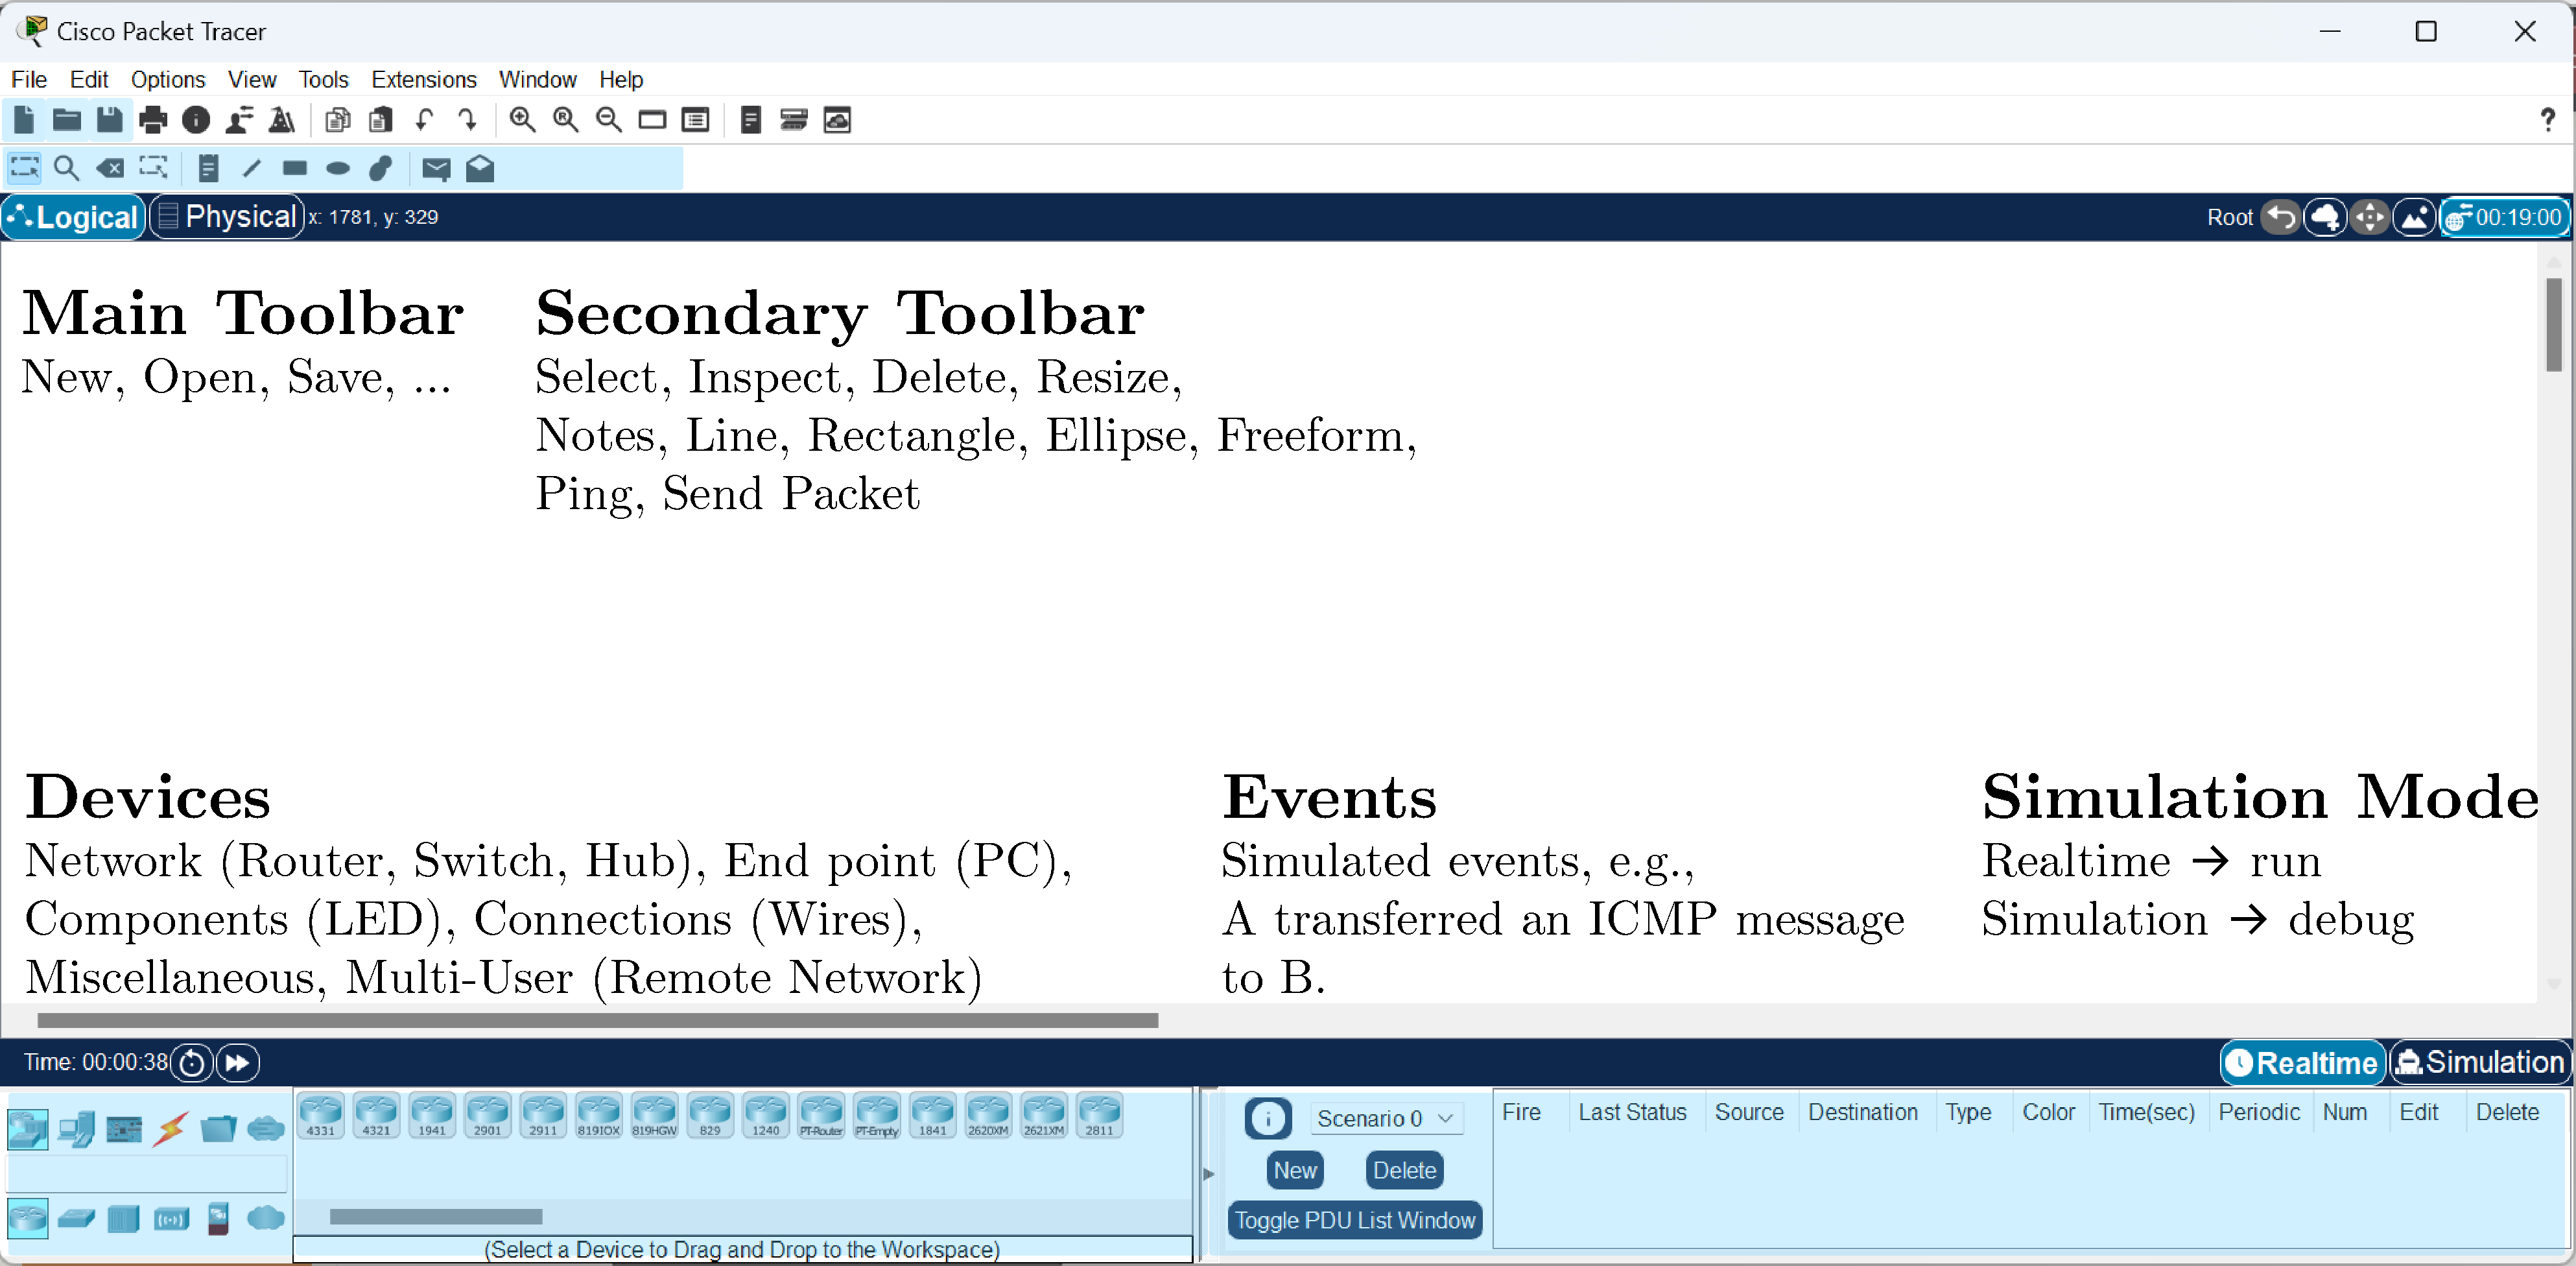
\includegraphics[width=\textwidth]{images/packet-tracer-empty.pdf}
    \caption{Cisco Packet Tracer First Screen}\label{fig:packet-tracer-empty}
\end{figure}

The goal of this section is to get you familiar with the Cisco Packet Tracer
software. We will create a simple network with three computers and a router.
Follow the steps below:

\begin{enumerate}
    \item Look at the bottom-left section where devices were listed. You should
          see a list of devices, including \menu{Router}, \menu{Switch},
          \menu{PC}, etc. Select the first one \menu{Network Devices}
          \icon{network-devices} After that, click
          on the hub icon \icon{hub} and drag a hub
          into the main window, it should look like \autoref{fig:hello-world-1}.
    \item After that, select the end devices
          \icon{end-devices} and drag 3 PC
          \icon{pc} into the main window. It should
          look like \autoref{fig:hello-world-2}.
    \item Finally, connect the hub to the three PCs. You can do this by clicking
          on the connections icon \icon{connections}
          and choose \menu{automatically choose connection type} icon as
          \icon{automatic-connections}; otherwise,
          we would need to understand all those connection types before we can
          do anything. After that, click on the hub and click on the first PC,
          then release the mouse button. Repeat this step for the other two PCs.
          It should look like \autoref{fig:hello-world-3}. To save you from
          selecting the automatic connection every time, you should press
          \keys{Ctrl} while you select, then you can connect the devices without
          selecting them repetitively.
\end{enumerate}

\begin{figure}
    \centering
    \begin{subfigure}[b]{0.3\textwidth}
        \centering
        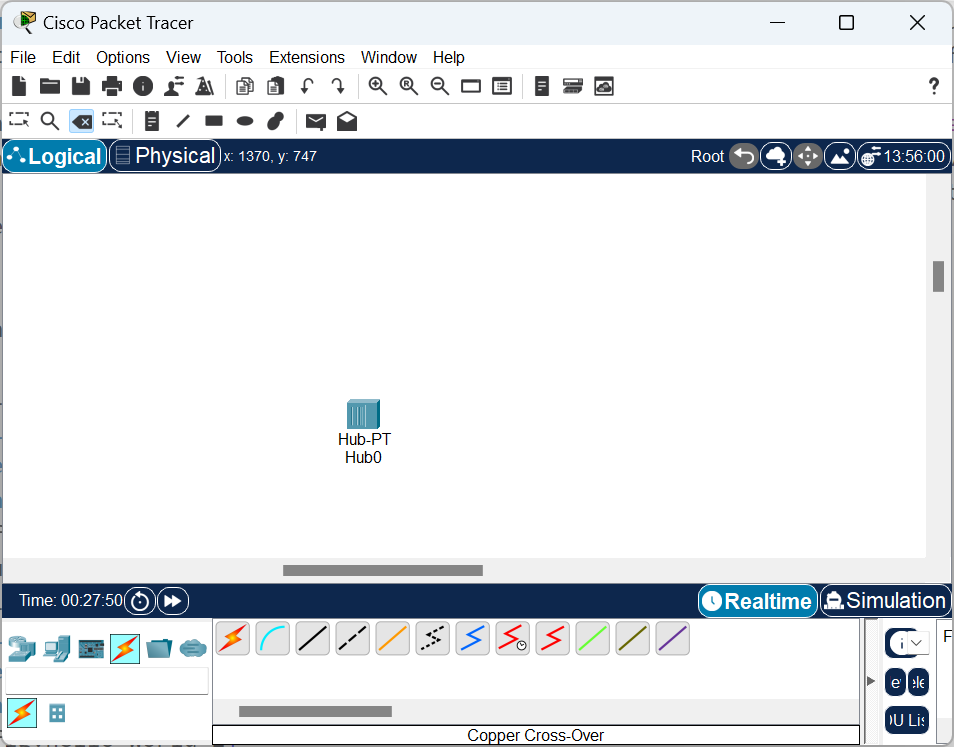
\includegraphics[width=\textwidth]{images/hello-world-1.png}
        \caption{Hub}\label{fig:hello-world-1}
    \end{subfigure}
    \begin{subfigure}[b]{0.3\textwidth}
        \centering
        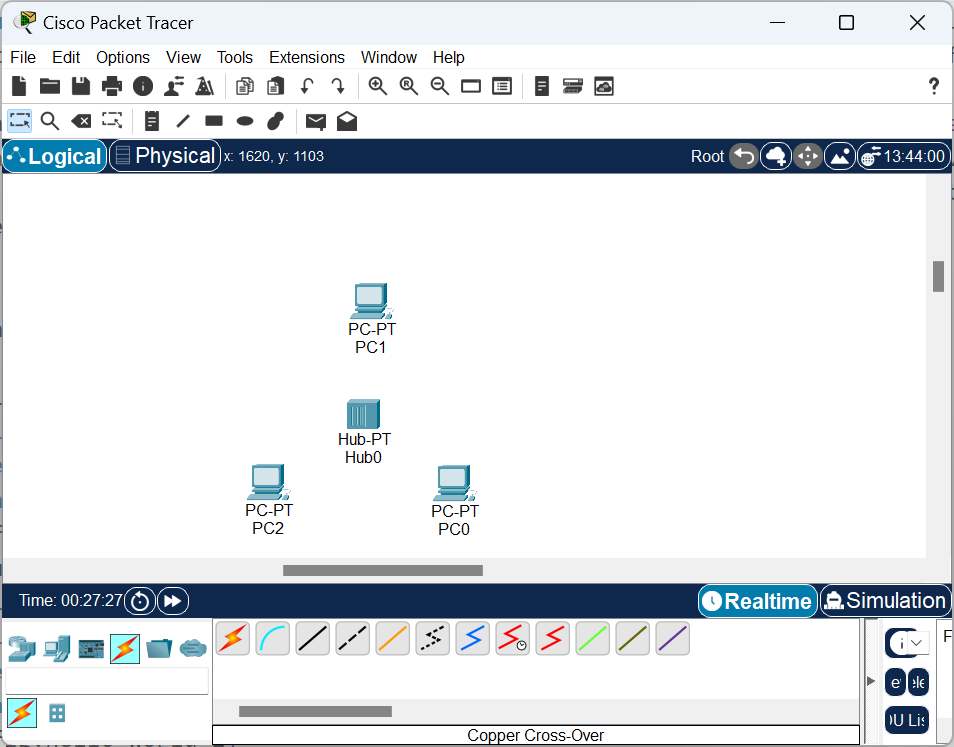
\includegraphics[width=\textwidth]{images/hello-world-2.png}
        \caption{PCs}\label{fig:hello-world-2}
    \end{subfigure}
    \begin{subfigure}[b]{0.3\textwidth}
        \centering
        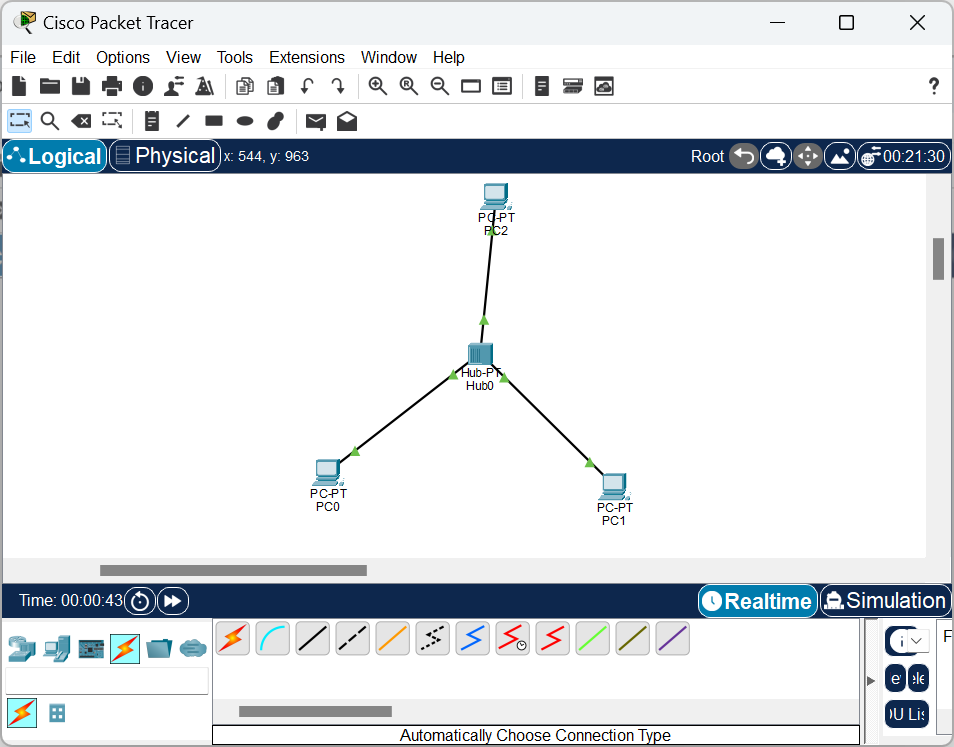
\includegraphics[width=\textwidth]{images/hello-world-3.png}
        \caption{Connections}\label{fig:hello-world-3}
    \end{subfigure}
    \caption{Setup Network Topology}\label{fig:hello-world-topology}
\end{figure}

After that, you should see a network topology as shown in \autoref{fig:hello-world-topology}. We will then configure this topology.

\subsubsection{Configure}

We will dive into the details of the IP address, subnet mask, and default
gateway later. For now, we will just use the default values with static IP
addresses. Follow the steps below:

\begin{enumerate}
    \item Click on any PC that we want to configure. You should see a window
          similar to \autoref{fig:hello-world-configure-1}. Click on the
          \menu{Desktop > IP Configuration} menu item. After that, set the IP
          configuration as \menu{Static} and type \mono!192.168.0.1! in the IPv4
          address field (\autoref{fig:hello-world-configure-2}). Left anything
          that is automatically generated as is.
    \item Repeat the same step for the other two PCs. The IP addresses should be
          incremented by one, i.e., \mono!192.168.0.2! and \mono!192.168.0.3!.
          This is necessary because distinct IP addresses in the same network
            are required for the network to work.
\end{enumerate}

\begin{figure}
    \begin{subfigure}[b]{0.48\textwidth}
        \centering
        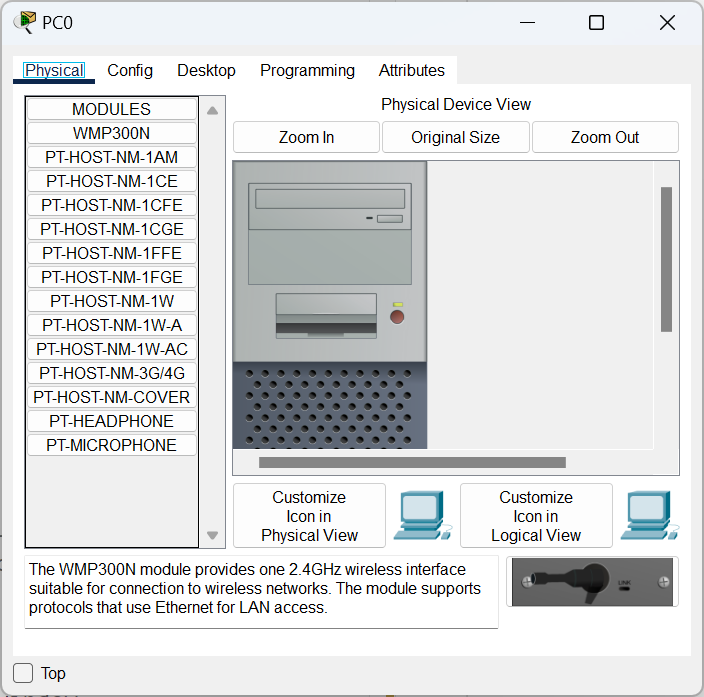
\includegraphics[width=\textwidth]{images/hello-world-configure-1.png}
        \caption{PC Configuration}\label{fig:hello-world-configure-1}
    \end{subfigure}
    \begin{subfigure}[b]{0.48\textwidth}
        \centering
        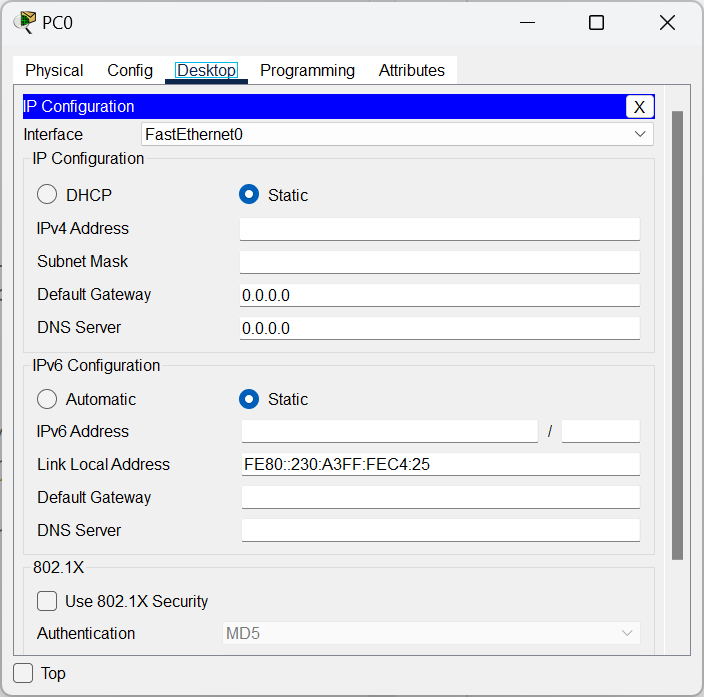
\includegraphics[width=\textwidth]{images/hello-world-configure-2.png}
        \caption{IP Configuration}\label{fig:hello-world-configure-2}
    \end{subfigure}
    \caption{Configure PC}\label{fig:hello-world-configure}
\end{figure}

\subsubsection{Ping}

Refer to \autoref{fig:packet-tracer-empty} for the initial window. Click on the
\icon{simple-pdu} icon and choose any 2 computers that we want to ping. After
that, nothing would be perceived on the screen
(\autoref{fig:hello-world-real-time}), except 1 more record is added to the
event list at the bottom-right corner of the program. Remove this record, and
switch to the simulation mode.

\begin{figure}
    \centering
    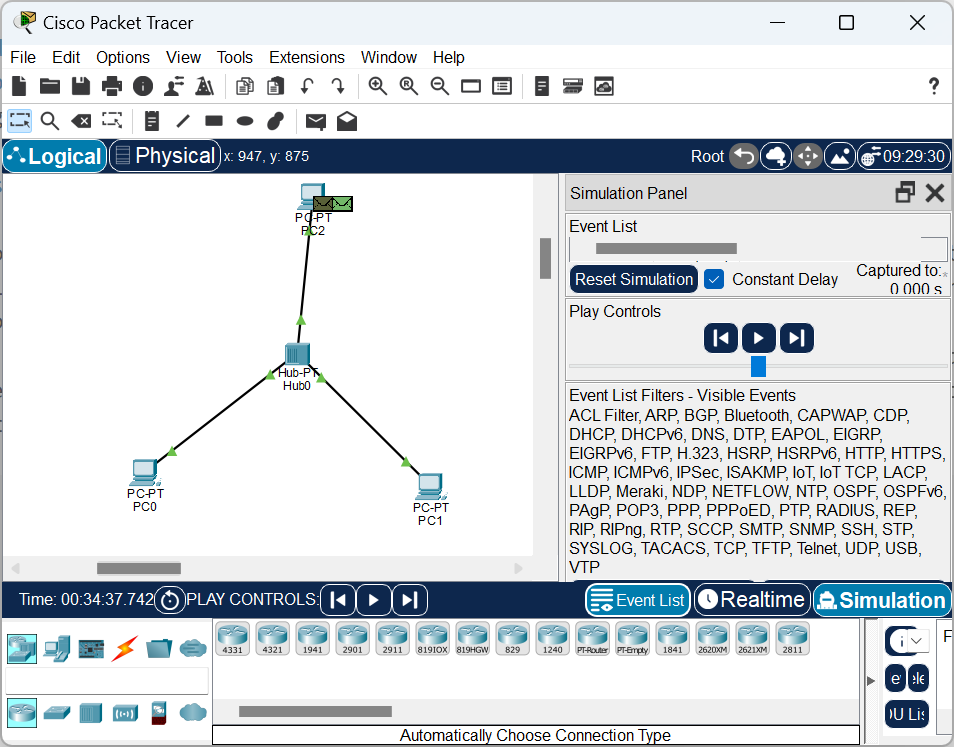
\includegraphics[width=0.5\textwidth]{images/hello-world-real-time.png}
    \caption{Real-Time Simulation}\label{fig:hello-world-real-time}
\end{figure}

In simulation mode, we can see the packets being sent and received in each step
by clicking on the \icon{step} icon; if we want to play to the end, click on the
\icon{play} icon. After that, we can see the packets being sent and received in
each step (\autoref{fig:hello-world-simulation}).

\begin{figure}
    \centering
    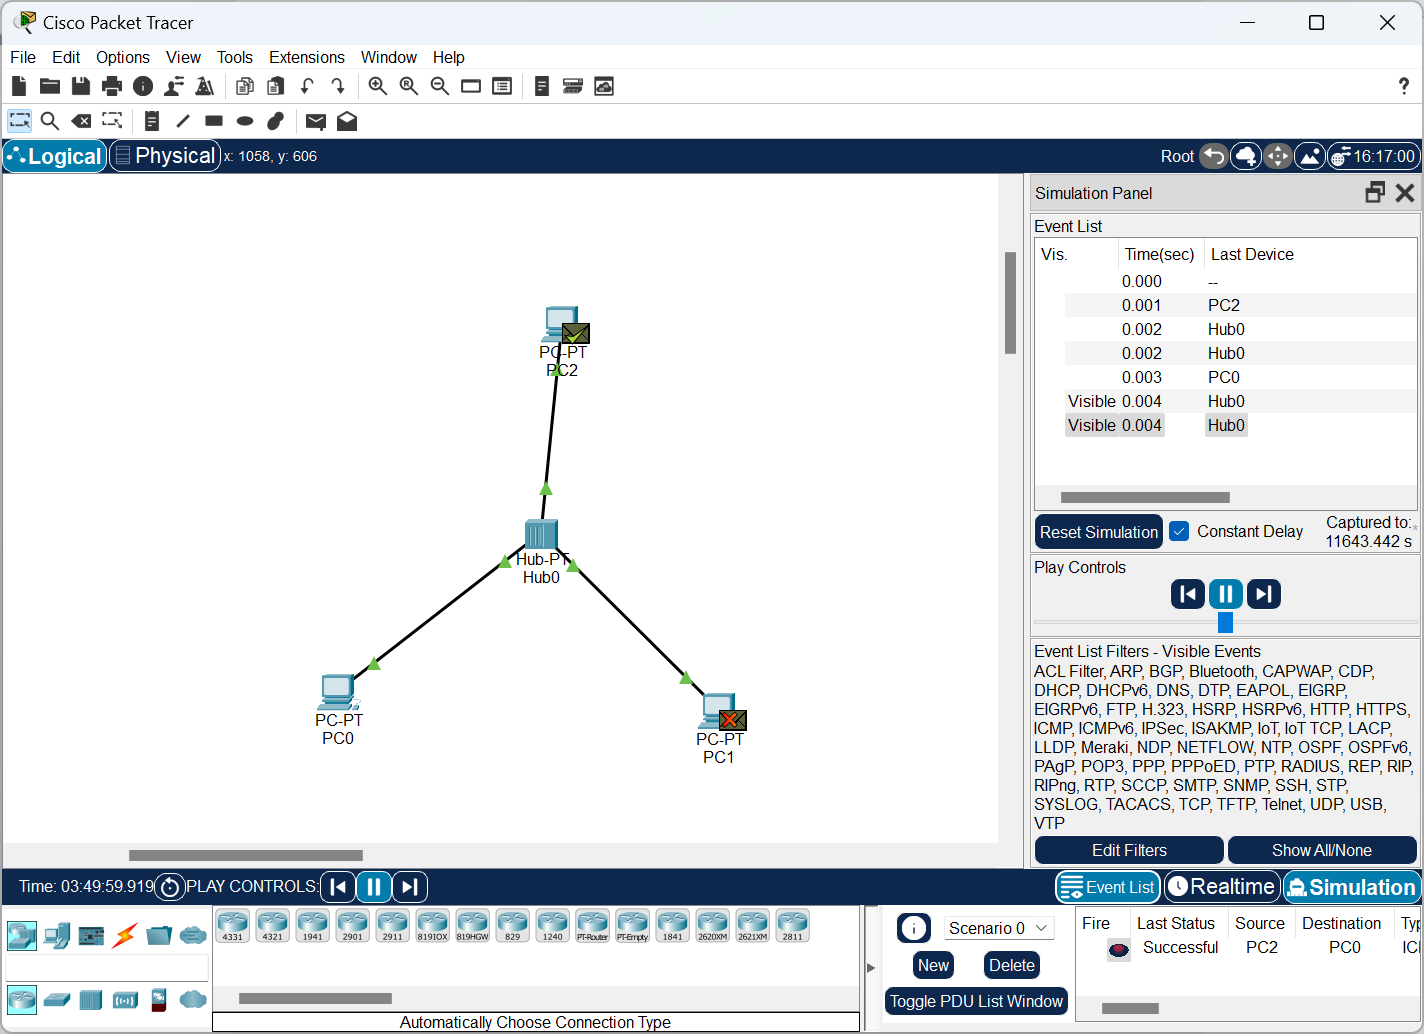
\includegraphics[width=0.5\textwidth]{images/hello-world-simulation.png}
    \caption{Simulation}\label{fig:hello-world-simulation}
\end{figure}

Assuming that we want to see how the exact structure of the packets being sent
and received, we can click on the event list shown at the right when the
simulation is running. For example, when we click on the first packet that is
sent by PC2, we can see the packet structure as shown in
\autoref{fig:hello-world-packet-structure}.

\begin{figure}
    \centering
    \begin{subfigure}[b]{0.48\textwidth}
        \centering
        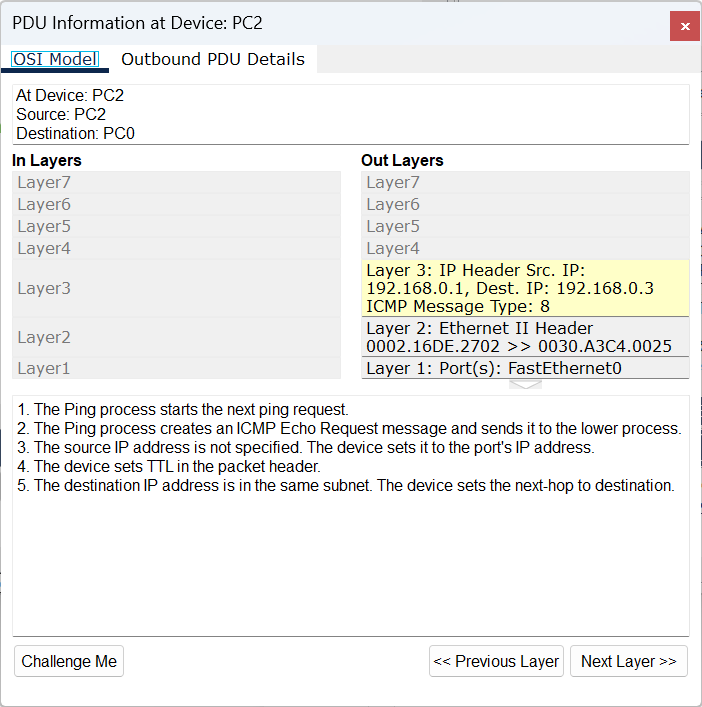
\includegraphics[width=\linewidth]{images/hello-world-packet-structure-1.png}
        \caption{Packet Structure 7-Layer}
    \end{subfigure}
    \begin{subfigure}[b]{0.48\textwidth}
        \centering
        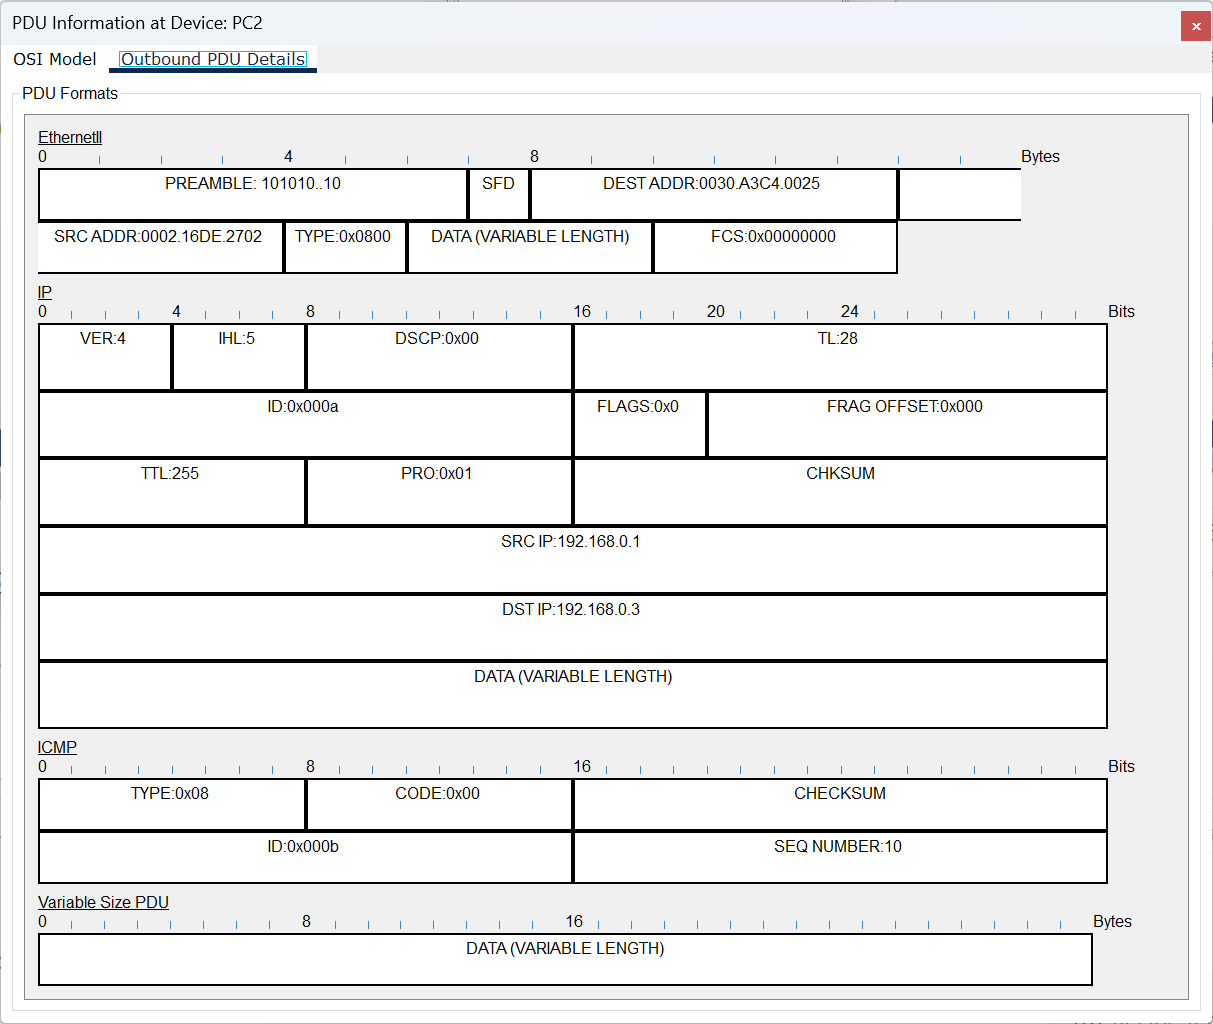
\includegraphics[width=\linewidth]{images/hello-world-packet-structure-2.png}
        \caption{Packet Structure Bytes}
    \end{subfigure}
    \caption{Packet Structure}\label{fig:hello-world-packet-structure}
\end{figure}
